\documentclass[math0540-lecture-notes.tex]{subfiles}
\begin{document}

\chapter{Operators on Inner Product Spaces}

\section{Self-Adjoint and Normal Operators}

We start with a review of linear functional.

\begin{definition}[Linear Functionals]{}
  A linear map from a vector space $V$ to a field $\F$ is a \textbf{linear functional}.
\end{definition}
For example, if $V$ is an inner product space, then for a fixed $v\in V$, \[
  \left<\cdot , v \right> :V\longrightarrow \F
,\] is a linear functional on $V$. Indeed, this is a linear map, since inner products are linear in
the first slot.

\begin{theorem}[Reisz Representation Theorem]{}
  Let $V$ be a finite-dimensional inner product space. Then given a linear functional $\phi:V\to
  \F$, there exists a unique vector $u\in V$ such that \[
    \phi(v)=\left<v,u \right> 
  \] for every $v\in V$.
\end{theorem}

\begin{example}
  Let $\phi:\R^2\to \R$ (with the usual Euclidean inner product) be given by $\phi(x,y)=x+y$. Reisz
  then tells us that there exists some $v\in \R^2$ such that \[
    \phi(x,y)=\left<(x,y),v \right> ~\text{for every}~(x,y)\in \R^2
  .\] Indeed, let $v=(1,1)$. Then $\left<(x,y),(1,1) \right> =x+y$.
\end{example}

Reisz Representation Theorem actually gives us a bijective function \[
  R:\mc{L}(V,\F)\longrightarrow V
.\] In other words, the space of all linear functionals from $V$ to $\F$ is bijective to $V$!
Indeed, $R$ is given by \[
  R(\phi)=\overline{\phi(e_1)}e_1+\ldots+\overline{\phi(e_n)}e_n=u
,\] where $\phi\in \mc{L}(V,\F)$ is a linear functional and $e_1,\ldots,e_n$ is an orthonormal basis
of $V$. $R$ is conjugate-linear, with linearity holding only when $\F$ is real.

Now, we move onto adjoints.
\begin{definition}[Adjoint, $T^*$]{}
  Suppose $T\in \mc{L}(V,W)$. The \textbf{adjoint} of $T$ is the function $T^*:W\to V$ such that \[
    \left<Tv,w \right> =\left<v,T^*w \right> 
  \] for every $v\in V$ and $w\in W$.

  Note that the left inner product is the \textbf{inner product on $W$}, while the right inner
  product is the \textbf{inner product on $V$}.
\end{definition}

But why does such a function $T^*$ actually exist, and why is it unique? Fix a $w\in W$, and
consider \[
  V\longrightarrow \F, v\mapsto \left<Tv,w \right> 
.\] This is a linear map from $V$ to $\F$, since it's just a linear map ($T$) composed with another
linear map ($\left<\cdot ,w \right> $). Then by the Reisz Representation Theorem, there is a unique
vector $T^*w\in V$ such that for all $v\in V$, \[
  \left<Tv,w \right> =\left<v,T^*w \right> 
.\] 

\begin{example}
  Define $T:\R^3\to \R^2$ by \[
    T(x_1,x_2,x_3)=(x_2+3x_3,2x_1)
  .\] Find a formula for $T^*$.
\end{example}
\begin{solution}
  Here $T^*\in \mc{L}(\R^2,\R^3)$. To compute $T^*$, fix a point $(y_1,y_2)\in \R^2$. Then for every
  $(x_1,x_2,x_3)\in \R^3$, we have
  \begin{align*}
    \left<(x_1,x_2,x_3),T^*(y_1,y_2) \right> &= \left<T(x_1,x_2,x_3),(y_1,y_2) \right>  \\ 
                                             &= \left<(x_2+3x_3,2x_1),(y_1,y_2) \right>  \\
                                             &= x_2y_1+3x_3y_1+2x_1y_2 \\
                                             &= \left<(x_1,x_2,x_3),(2y_2,y_1,3y_1) \right>
  .\end{align*} Thus \[
  T^*(y_1,y_2)=(2y_2,y_1,3y_1)
  .\] 
\end{solution}
\begin{example}
  Fix $u\in V$ and $x\in W$. Define $T\in \mc{L}(V,W)$ by \[
    Tv=\left<v,u \right> x
  \] for every $v\in V$. Find a formula for $T^*$.
\end{example}
\begin{solution}
  Fix $w\in W$. Then for every $v\in V$, we have
  \begin{align*}
    \left<v,T^*w \right> &= \left<Tv,w \right>  \\
    &= \left<\left<v,u \right> x,w \right>  \\
    &= \left<v,u \right> \left<x,w \right>  \\
    &= \left<v,\left<w,x \right> u \right> 
  .\end{align*} Thus \[
    T^*w=\left<w,x \right> u
  .\] 
\end{solution}

In the above examples, $T^*$ was not only a function, but indeed a linear map. This is true in
general.
\begin{proposition}[Adjoint is Linear]{}
  If $T\in \mc{L}(V,W)$, then $T^*\in \mc{L}(W,V)$ (equivalently, $T^*$ is a linear map).
\end{proposition}
\begin{proof}[Proof]
  Suppose $T\in \mc{L}(V,W)$. Fix $w_1,w_2\in W$. If $v\in V$, then
  \begin{align*}
    \left<v,T^*(w_1+w_2) \right>&= \left<Tv,w_1+w_2 \right>  \\
    &= \left<Tv,w_1 \right> +\left<Tv,w_2 \right>  \\
    &= \left<v,T^*w_1 \right> +\left<v,T^*w_2 \right>  \\
    &=\left<v,T^*w_1+T^*w_2 \right> 
  .\end{align*}
  Hence $T^*(w_1+w_2)=T^*w_1+T^*w_2$. A similar computation follows for $\lambda\in \F$; thus
  $T^*\in \mc{L}(W,V)$, as desired.
\end{proof}

Let's look at some properties of the adjoint.
\begin{proposition}[Properties of Adjoints]{}
  \begin{enumerate}
    \item $(S+T)^*=S^*+T^*$ for all $S,T\in \mc{L}(V,W)$;
    \item $\left( \lambda T \right)^*=\overline{\lambda}T^* $ for every $\lambda\in \F$, $T\in
      \mc{L}(V,W)$;
    \item $(T^*)^*=T$ for all $T\in \mc{L}(V,W)$;
    \item $I^*=I$, where $I$ is the identity operator on $V$;
    \item $(ST)^*=T^*S^*$ for all $T\in \mc{L}(V,W)$ and $S\in \mc{L}(W,U)$ (here $U$ is another
      inner product space over $\F$).
  \end{enumerate}
\end{proposition}
\begin{proof}[Proof]
  \begin{enumerate}
    \item Suppose $S,T\in \mc{L}(V,W)$. If $v\in V$ and $w\in W$, then
      \begin{align*}
        \left<v,(S+T)^*w \right> &= \left<(S+T)v,w \right>  \\
                                 &= \left<Sv,w \right>+\left<Tv,w \right>   \\
                                 &= \left<v,S^*w \right> +\left<v,T^*w \right>  \\
                                 &=\left<v,S^*w+T^*w \right>  
       .\end{align*} Hence $(S+T)^*=S^*+T^*$, as desired.
     \item Suppose $\lambda\in \F$ and $T\in \mc{L}(V,W)$. If $v\in V$ and $w\in W$, then \[
           \left<v,(\lambda T)^*w \right> =\left<\lambda Tv,w \right> =\lambda\left<Tv,w \right>
           =\left<v,\overline{\lambda} T^*w\right> 
       ,\] as desired.
     \item Suppose $T\in \mc{L}(V,W)$. Then \[
           \left<w,(T^*)^*v \right> =\left<T^*w,v \right> =\overline{\left<v,T^*w
           \right>}=\overline{\left<Tv,w \right> }=\left<w,Tv \right> 
       ,\] as desired.
     \item If $v,u\in V$, then \[
       \left< v,I^*u \right> =\left<Iv,u \right> =\left<v,u \right> 
     .\] Hence $I^u=u$, as desired.
   \item Suppose $T\in \mc{L}(V,W)$ and $S\in \mc{L}(W,U)$. If $v\in V$ and $u\in U$, then \[
       \left<v,(ST)^*u \right> =\left<STv,u \right> =\left<Tv,S^*u \right> =\left<v,T^*S^*u \right> 
     .\] Thus $(ST)^*=T^*S^*$, as desired.
  \end{enumerate}
\end{proof}

We now inspect relationships between the null space and the range of a linear map and its adjoint.
\begin{proposition}[Null Space and Range of $T^*$]{}
  Suppose $T\in \mc{L}(V,W)$. Then
  \begin{enumerate}
    \item $\Null{T^*}=(\range{T})^\bot$
    \item $\range{T^*}=(\Null{T})^\bot$
    \item $\Null{T}=(\range{T^*})^\bot$
    \item $\range{T}=(\Null{T^*})^\bot$
  \end{enumerate}
\end{proposition}
\begin{proof}[Proof]
  Let $w\in W$. Then
  \begin{align*}
    w\in \Null{T^*}&\iff T^*w=0\\
                   &\iff \left<v,T^*w \right> =0 ~\text{for all}~v\in V\\
                   &\iff \left<Tv,w \right> =0~\text{for all}~v\in V\\
                   &\iff w\in (\range{T})^\bot
  .\end{align*}
  Thus $\Null{T^*}=(\range{T})^\bot$. Taking the orthogonal complement of both sides gives us \[
    \range{T}=(\Null{T^*})^\bot
    ,\] proving (d). Replacing $T^*$ with $T$ from (a) gives us (c): \[
    \Null{T}=(\range{T^*})^\bot
  ,\] and similarly for (b) and (d).

\end{proof}

Finally, let us inspect the matrices of $T$ and $T^*$.
\begin{definition}[Conjugate Transpose]{}
  The \textbf{conjugate transpose} of an $m\times n$ matrix is the $n\times m$ matrix obtained by
  interchanging the rows and columns, then taking the complex conjugate of each entry.
\end{definition}

This next result shows how to compute the matrix of $T^*$ given the matrix of $T$. Note that
\textbf{this only applies when dealing with orthonormal bases}!

\begin{proposition}[Matrix of $T^*$]{}
  Let $T\in \mc{L}(V,W)$. Suppose $e_1,\ldots,e_n$ is an orthonormal basis of $V$ and
  $f_1,\ldots,f_m$ is an orthonormal basis of $W$. Then \[
    \mc{M}(T^*,(f_1,\ldots,f_m),(e_1,...,e_n))
  \] is the conjugate transpose of \[
  \mc{M}(T,(e_1,\ldots,e_n), (f_1,\ldots,f_m))
  .\] 
\end{proposition}
\begin{proof}[Proof]
  Denote $\mc{M}(T)$ and $\mc{M}(T^*)$, instead of their longer expressions with the specified
  orthonormal bases.

  Let's calculate $\mc{M}(T)_{j,k}$ and $\mc{M}(T^*)_{k,j}$; if they are conjugates, we are done.
  Writing \[
    Te_k=\left<Te_k,f_1 \right>f_1+\ldots+\left<Te_k,f_m \right> f_m 
  \] (since $f_1,\ldots,f_m$ is an orthonormal basis for $W$, and $Te_k\in W$) shows that \[
    \mc{M}(T)_{j,k}=\left<Te_k,f_j \right> =\left<e_k,T^*f_j \right> 
    \] (since the $j,k$-th entry of $\mc{M}(T)$ is the coefficient of $f_j$ of the basis
    representation of $Te_k$). Similarly, writing \[
    T^*f_j=\left<T^*f_j,e_1 \right> e_1+\ldots+\left<T^*f_j,e_n \right> e_n
  \] gives us \[
    \mc{M}(T^*)_{k,j}=\left<T^*f_j,e_k \right> =\overline{\left<e_k,T^*f_j \right>
    }=\overline{\left<Te_k,f_j \right> }
  ,\] the complex conjugate of $\left<Te_k,f_j \right> =\mc{M}(T)_{j,k}$, as desired.
\end{proof}

\subsection{Self-Adjoint Operators}
We now focus on operators on inner product spaces.
\begin{definition}[Self-Adjoint]{}
  An operator $T\in \mc{L}(V)$ is called \textbf{self-adjoint} if $T=T^*$; that is, $T\in \mc{L}(V)$
  is self-adjoint if and only if \[
    \left<Tv,w \right> =\left<v,Tw \right> 
  \] for all $v,w\in V$.
\end{definition}

From above, we know that the adjoint's matrix representation is the complex conjugate of the
operator. Thus, we know that an operator $T$ is self-adjoint if and only if $\mc{M}(T)$ is equal to
its conjugate transpose. That is, \[
  \mc{M}(T)^T=\overline{\mc{M}(T)}
.\] 

\begin{definition}[Adjoint of a Matrix]{}
  Given an $n\times n$ matrix $A$, define its adjoint $A^*=\overline{A}$; that is, for an operator
  $T\in \mc{L}(V)$, the matrix of its adjoint is the adjoint of its matrix (with respect to an
  orthonormal basis).
\end{definition}

Intuitively, let's start with the real case $\F=\R$. A real operator $T\in \mc{L}(V)$ is then
self-adjoint if and only if it has a \textit{symmetric} matrix with respect to an orthonormal basis.
In the complex case, you can get some intuition in the one-dimensional case; the space of operators
$\mc{L}(V)$ would be identified with $1\times 1$ complex matrices, or equivalently, the complex
numbers $\C$. Then an operator over a complex inner product space is self-adjoint if and only if its
matrix is \textit{real}.

In general, it's helpful to think of self-adjoint operators among all operators, as analogous to
real numbers among all complex numbers.

\begin{remark}
  Sometimes, mathematicians will use the term \textbf{Hermitian} instead of self-adjoint, in honor
  of French mathematician Charles Hermite. Generally, self-adjoint will be used to describe
  operators, while Hermitian will be used to describe matrices.
\end{remark}

Let's now inspect some important properties of self-adjoint operators.
\begin{proposition}[Eigenvalues of Self-Adjoint Operators are Real]{}
  Every eigenvalue of a self-adjoint operator is real.
\end{proposition}
\begin{proof}[Proof]
  Suppose $T\in \mc{L}(V)$ is a self-adjoint operator, and let $\lambda\in \F$ be an eigenvalue of
  $T$. Let $v\in V$ be a non-zero vector such that $Tv=\lambda v$. Then \[
    \lambda\|v\|^2=\left<\lambda v,v \right> =\left< Tv,v\right> =\left<v,Tv \right>
    =\left<v,\lambda v \right> =\overline{\lambda}\|v\|^2
  .\] Since $\|v\|^2>0$ (since $v$ non-zero), we have $\lambda=\overline{\lambda}$, and so $\lambda$
  is real.
\end{proof}
Later, we will see a different proof using the Spectral Theorem.

This next result will be stated without proof, and used in the following proposition. See Axler 7.14
(p. 210) for a proof. Note that this result is false for real inner product spaces; the operator
$T\in \mc{L}(\R^2)$ of a counter-clockwise rotation of $90^{\circ}$ is a counterexample.
\begin{proposition}{}
  Suppose $V$ is a complex inner product space and $T\in \mc{L}(V)$, and suppose \[
    \left<Tv,v \right> =0
  \] ($Tv$ is orthogonal to $v$ for every $v\in V$). Then $T=0$.
\end{proposition}

We explained previously how self-adjoint operators are analogous to real numbers in a complex field.
This formalizes the result.

\begin{proposition}{}
  Suppose $V$ is a complex inner product space and $T\in \mc{L}(V)$. Then $T$ is self-adjoint if and
  only if \[
    \left<Tv,v \right> \in \R
  \] for every $v\in V$.
\end{proposition}
\begin{proof}[Proof]
  Suppose $\left<Tv,v \right> \in \R$ for every $v\in V$. Then \[
    0=\left<Tv,v \right> -\overline{\left<Tv,v \right> }=\left<Tv,v \right> -\left<v,Tv \right>
    =\left<Tv,v \right> -\left<T^*v,v \right> =\left<(T-T^*)v,v \right> 
  .\] So, $\left<(T-T^*)v,v \right> =0$ for every $v\in V$, which means $T-T^*=0$ (from above); in
  other words, $T=T^*$, and $T$ is self-adjoint.

  Conversely, suppose $T$ is self-adjoint. Then from above, $\left<(T-T^*)v,v \right> =0$, so \[
  \left<Tv,v \right> -\overline{\left<Tv,v \right> }=0
  \] for every $v\in V$. This means that $\left<Tv,v \right> \in \R$ for every $v\in V$, as desired.
\end{proof}

Note that the above result is clearly not true for any real inner product space; simply consider a
non-self-adjoint operator on the space.

This final result will be stated without proof; see Axler 7.16 (p. 211). Essentially, the result of
a self-adjoint operator $Tv$ is not orthogonal to the original $v\in V$ unless $T=0$.
\begin{proposition}{}
  Suppose $T\in \mc{L}(V)$ is a self-adjoint operator with \[
    \left<Tv,v \right> =0
  \] for all $v\in V$. Then $T=0$.
\end{proposition}

\subsection{Normal Operators}
\begin{definition}[Normal Operators]{}
  An operator on an inner product space is \textbf{normal} if it commutes with its adjoint; that is,
  $T\in \mc{L}(V)$ is normal if \[
    TT^*=T^*T
  .\] 
\end{definition}

Obviously, every self-adjoint operator is normal, since $T$ self-adjoint means $T=T^*$. As we'll see
later, normal operators are of special importance in spectral theory.

Let's now characterize normal operators.
\begin{proposition}{}
  An operator $T\in \mc{L}(V)$ is normal if and only if \[
    \|Tv\|=\|T^*v\|
  \] for all $v\in V$.
\end{proposition}
\begin{proof}[Proof]
  Suppose $T\in \mc{L}(V)$. Note that
  \begin{align*}
    T ~\text{is normal}~&\iff T^*T-TT^*=0\\
                        &\iff \left<(T^*T-TT^*)v,v \right>=0 ~\text{for all}~v\in V\\
                        &\iff \left<T^*Tv,v \right> =\left<TT^*v,v \right> ~\text{for all}~v\in V\\
                        &\iff \left<Tv,Tv \right> =\left<T^*v,T^*v \right> ~\text{for all}~v\in V\\
                        &\iff \|Tv\|^2=\|T^*v\|^2
  ,\end{align*} as desired.
  The second equivalence comes because if $T$ is a self-adjoint operator and $\left<Tv,v \right>
  =0$, then $T=0$ (the converse comes trivially); one can check, using adjoint properties, that
  $T^*T-TT^*$ is self-adjoint.
\end{proof}
Using this, we can glean some information about the eigenvalues of normal operators.
\begin{proposition}{}
  Suppose $T\in \mc{L}(V)$ is normal and $v\in V$ is an eigenvector of $T$ with eigenvalue
  $\lambda$. Then $v$ is also an eigenvector of $T^*$ with eigenvalue $\overline{\lambda}$. 
\end{proposition}
\begin{proof}[Proof]
  Because $T$ is normal, so is $T-\lambda I$ (to see this, consider its adjoint
  $T^*-\overline{\lambda}I$; verify then that this is normal). From above, we have \[
    0 = \|(T-\lambda I)v\|=\|(T-\lambda I)^*v\|=\|(T^*-\overline{\lambda}I)v\|
  .\] Hence $v$ is an eigenvector of $T^*$ with eigenvalue $\overline{\lambda}$, as desired (recall
  that a vector $v\in V$ is an eigenvector if and only if $v\in \Null{(T-\lambda I)}$).
\end{proof}

Essentially, that is, normal operators and their adjoints have the same eigenvectors. 

This next result applies in particular to self-adjoint operators, since all self-adjoint operators
are nomal.
\begin{proposition}[Orthogonal Eigenvectors for Normal Operators]{}
  Suppose $T\in \mc{L}(V)$ is normal. Then eigenvectors of $T$ corresponding to distinct eigenvalues
  are orthogonal.
\end{proposition}
\begin{proof}[Proof]
  Suppose $\alpha,\beta \in \F$ are distinct eigenvalues of $T$, with corresponding eigenvectors
  $u,v\in V$. Thus $Tu=\alpha u$ and $Tv=\beta v$. From above, we have $T^*v=\overline{\beta}v$;
  thus 
  \begin{align*}
    (\alpha-\beta)\left<u,v \right> &= \left<\alpha u,v \right>-\left<u,\overline{\beta}v \right>   \\
                                    &= \left<Tu,v \right> -\left<u,T^*v \right>  \\
                                    &= 0
  .\end{align*} Since $\alpha\neq \beta$, the above equation implies $\left<u,v \right> =0$; thus
  $u$ and $v$ are orthogonal.
\end{proof}

\section{The Spectral Theorem}
One of the cornerstones of inner product spaces, and indeed linear algebra, is the Spectral Theorem.
Since the results are dependent on the choice of field $\F=\R$ or $\C$, we break the Spectral
Theorem into two pieces. We start with the complex case, since as is often the case in linear
algebra, the complex case is easier to deal with than the real case.

\subsection{The Complex Spectral Theorem}
The key part of the Complex Spectral Theorem states that if $\F=\C$ and $T\in \mc{L}(V)$ is normal,
then $T$ has a diagonal matrix with respect to some orthonormal basis of $V$. For example, consider
the normal operator $T\in \mc{L}(\C^2)$, with matrix \[
  \begin{pmatrix} 2&-3\\3&2 \end{pmatrix} 
\] (verify that despite not being self-adjoint, this operator is normal!). One can check that \[
\frac{(i,1)}{\sqrt{2}},\ \frac{(-i,1)}{\sqrt{2}}
\] is an orthonormal basis for $\C^2$ consisting of eigenvectors of $T$, and with respect to this
basis, the matrix of $T$ is the diagonal matrix \[
  \begin{pmatrix} 2+3i&0\\0&2-3i \end{pmatrix} 
.\] 

\begin{theorem}[Complex Spectral Theorem]{}
  Suppose $\F=\C$ and $T\in \mc{L}(V)$. Then the following are equivalent:
  \begin{enumerate}
    \item $T$ is normal.
    \item $V$ has an orthonormal basis consisting of eigenvectors of $T$.
    \item $T$ has a diagonal matrix with respect to some orthonormal basis of $V$.
  \end{enumerate}
\end{theorem}
\begin{proof}[Proof]
  The equivalence of (b) and (c) holds $T$ diagonalizable with respect to some basis (which, by
  Gram-Schmidt, can be converted to an orthonormal basis) if and only if $V$ has a basis consisting
  of eigenvectors of $T$.

  Now, suppose (c) holds, so $T$ has a diagonal matrix with respect to some orthonormal basis of
  $V$; the matrix of $T^*$ (with respect to the same basis) is the conjugate transpose of
  $\mc{M}(T)$; hence $T^*$ also has a diagonal matrix. Since any two diagonal matrices commute, $T$
  thus commutes with $T^*$, so $T$ is normal.

  Conversely, suppose $T$ is normal. By Schur's Theorem, there is an orthonormal basis
  $e_1,\ldots,e_n\in V$ with respect to which $T$ has an upper-triangular matrix. Thus we can write
  \[
    \mc{M}(T)=\begin{pmatrix} a_{1,1}&\cdots&a_{1,n}\\ &\ddots&\vdots\\0& &a_{n,n} \end{pmatrix} 
  .\] Let's see why this is actually a diagonal matrix.

  From this matrix, we have $\|Te_1\|^2=\left| a_{1,1} \right| ^2$, and \[
    \|T^*e_1\|^2=\|a_{1,1}\|^2+\ldots+\|a_{1,n}\|^2
  .\] Since $T$ is normal, we have $\|Te_1\|=\|T^*e_1\|$; but this then implies that $a_{j,n}=0$ for
  all $1<j\le n$.

  Continuing in this fashion for $Te_2,\ldots,Te_n$, we see that $\mc{M}(T)$ is actually a diagonal
  matrix; thus (c) holds.
\end{proof}

Essentially, if $T$ is a normal operator, then $T$ has an orthonormal basis consisting of
eigenvectors of $T$.

\subsection{The Real Spectral Theorem}

We'll start with some preliminary results, which apply to both real and complex inner product
spaces, in order to build up to the Real Spectral Theorem.

Let's start with a fact about factoring.
\begin{proposition}{}
  Let $p(x)=a_0+a_1x+\ldots+a_nx^n$ with $a_0,...,a_n\in \R$. Then $p(x)$ factors uniquely (up to
  ordering) into a product of the form \[
    p(x)=c(x^2+b_1x+c_1)\ldots(x^2+b_Mx+c_M)(x-\lambda_1)\ldots(x-\lambda_m)
  ,\] where all of the numbers $c,b_i,c_i,\lambda_j\in \R$, and $b_i^2-4c_i<0$. Thus, the real roots
  of $p(x)$ are exactly $\lambda_1,\ldots,\lambda_m$ (note that this doesn't necessarily guarantee
  any real roots; no real roots simply means $m=0$).
\end{proposition}
\begin{proof}[Proof]
  For a proof, see Axler 4.17 (p.128).
\end{proof}
This next result is intuitively true; one could even discover its proof by thinking about quadratic
polynomials with real coefficients. Specifically, suppose $b,c\in \R$ with $b^2<4ac$, and let $x$ be
a real number. Then \[
  x^2+bx+c=\left( x+\frac{b}{2} \right) ^2+\left( c-\frac{b^2}{4} \right) >0
\] (to obtain this, complete the square). In particular, $x^2+bx+c$ is an invertible real number (a
convoluted way of saying that it is not $0$). Replacing $x$ with a self-adjoint operator (recall our
heuristic of the analogy between real numbers and self-adjoint operators!), we get the following
result.
\begin{proposition}{}
  Suppose $T\in \mc{L}(V)$ and $b,c\in \R$ are such that $b^2<4ac$. Then \[
    T^2+bT+cI
  \] is invertible.
\end{proposition}
\begin{proof}[Proof]
  We claim that for all non-zero $v\in V$, we have \[
    \left<(T^2+bT+cI)v,v \right> \neq 0
  .\] Recall that $\left<u,v \right> =0$ only when $u$ or $v$ is $0$; thus, proving the above
  equation shows that $T^2+bT+cI$ has a trivial null space, which means that it's injective (and
  hence invertible).

  From completing the square above, we get \[
    T^2+bT+cI=\left( T+\frac{b}{2}I \right) ^2+\left( c-\frac{b^2}{4} \right) I
  .\] Moreover, note that $T+\frac{b}{2}I$ is self-adjoint since $T$ is (think about its matrix with
  respect to an orthonormal basis; since $\frac{b}{2}$ is real, its complex conjugate is the same).
  We then have
  \begin{align*}
    \left<(T^2+bT+cI)v,v \right> &=\left<(T^2+\frac{b}{2}I)^2v,v \right> +\left<(c-\frac{b^2}{4})v,v
    \right>\\
                                 &=\left<(T+\frac{b}{2}I)v,(T+\frac{b}{2}I)v
                                 \right>+(c-\frac{b^2}{4})\left<v,v \right> \\
                                 &>0
  ,\end{align*}where the third equality comes because $T+\frac{b}{2}I$ is self-adjoint. Thus
  $T^2+bT+cI$ is invertible.
\end{proof}

For the next result, remember the context; we've already shown that every operator on a complex
vector space has an eigenvector. However, this isn't always true for real vector spaces. We now show
that this will be true if $T$ is a self-adjoint operator.
\begin{proposition}[Self-Adjoint Operators have Eigenvalues]{}
  Suppose $V\neq \{ 0 \}$, and $T\in \mc{L}(V)$ is a self-adjoint operator. Then $T$ has an
  eigenvalue.
\end{proposition}
\begin{proof}[Proof]
  Assume that $V$ is a real vector space, and let $n=\dim{V}$. Choose $v\in V$ with $v\neq 0$; then
  \[
    v,Tv,\ldots,T^nv
  \] cannot be linearly independent, since $V$ has dimension $n$ and we have $n+1$ vectors. Thus for
  some real numbers $a_0,\ldots,a_n$ not all $0$, we have \[
    a_0+a_1Tv+\ldots+a_nT^nv=\textbf{0}
  .\] Rewriting, we have $p(z)=a_0+a_1z+\ldots+a_nz^n$; then $p(T)(v)=\textbf{0}$. Factoring, we
  have \[
    \textbf{0}=c(T^2+b_1T+c_1I)\ldots(T^2+b_MT+c_MI)(T-\lambda_1I)\ldots(T-\lambda_mI)v
  \] for real numbers $c,b_i,c_i,\lambda_j$ and $b_i^2<4c_i$. However, all the operators
  $T^2+b_iT+c_iI$ are invertible; thus one of the $T-\lambda_jI$ must be not invertible; that is,
  $\lambda_j$ is an eigenvalue for $T$.
\end{proof}

We prove one last result before approaching the Real Spectral Theorem.
\begin{proposition}[]{}
  Suppose $T\in \mc{L}(V)$ is self-adjoint and $U$ is a subspace of $V$ that is invariant under $T$
  (that is, every $u\in U$ has $Tu\in U$). Then
  \begin{enumerate}
    \item $U^{\bot}$ is invariant under $T$;
    \item $T|_U\in \mc{L}(U)$ is self-adjoint;
    \item $T|_{U^{\bot}}\in \mc{L}(U^{\bot})$ is self-adjoint.
  \end{enumerate}
\end{proposition}
\begin{proof}[Proof]
  For (a), suppose $v\in U^{\bot}$, and let $u\in U$. Then \[
    \left<Tv,u \right> =\left<v,Tu \right> =0
  ,\] where the first equality holds because $T$ is self-adjoint and the second because $U$ is
  invariant under $T$, meaning $Tu\in U$, and $v\in U^{\bot}$, meaning $v$ is orthogonal to any
  $u\in U$. Since this means $\left<Tv,u \right> =0$ for any $u\in U$, we must have $Tv\in
  U^{\bot}$; thus $U^{\bot}$ is invariant under $T$.

  For (b), note that if $u,v\in U$, then \[
    \left<(T|_U)u,v \right> =\left<Tu,v \right> =\left<u,Tv \right> =\left<u,(T|_U)v \right> 
  .\] Thus $T|_U$ is self-adjoint. A similar process proves (c).
\end{proof}

Now, we can finally proceed to the Real Spectral Theorem.
\begin{theorem}[Real Spectral Theorem]{}
  Suppose $\F=\R$ and $T\in \mc{L}(V)$. Then the following are equivalent:
  \begin{enumerate}
    \item $T$ is self-adjoint.
    \item $V$ has an orthonormal basis consisting of eigenvectors of $T$.
    \item $T$ has a diagonal matrix with respect to some orthonormal basis of $V$.
  \end{enumerate}
\end{theorem}
\begin{proof}[Proof]
  (b) and (c) are clearly equivalent. Suppose (c) holds, so $T$ has a diagonal matrix with respect
  to some orthonormal basis of $V$. A diagonal matrix equals its transpose, so $T=T^*$; that is, $T$
  is self-adjoint. Thus (c) implies (a).

  Suppose that $T$ is self-adjoint. We proceed by induction on $\dim{V}$. If $\dim{V}=1$, then
  clearly $V$ has an orthonormal basis of eigenvectors of $T$; so, assume $\dim{V}>1$ and that the
  theorem holds for all real inner product spaces of a smaller dimension.

  Let $u$ be an eigenvector of $T$ with $\|u\|=1$; from before, we've guaranteed that every
  self-adjoint operator has an eigenvector, which can then be scaled to normalize it. Let
  $U=\Span{(u)}$. Then $U$ is a $1$-dimensional subspace of $V$ that is invariant under $T$.
  However, from before we get that $T$ restricted to $U^{\bot}$, $T|_{U^{\bot}}\in
  \mc{L}(U^{\bot})$, is self-adjoint.

  Since $\dim{U^{\bot}}=n-1$ (recall that $U\oplus U^{\bot}=V$), our induction hypothesis tells us
  that there is an orthonormal basis of $U^{\bot}$ consisting of eigenvectors of $T|_{U^{\bot}}$
  (since $T|_{U^{\bot}}$ is a self-adjoint operator on $U^{\bot}$), and thus eigenvectors of $T$.
  Adjoining $u$ to this orthonormal basis of $U^{\bot}$ gives an orthonormal basis of $V$ consisting
  of eigenvectors of $T$, completing the proof.
\end{proof}

\section{Positive Operators and Isometries}
\subsection{Positive Operators}

Let's start with a preliminary definition.
\begin{definition}[Square Root]{}
  Let $T\in \mc{L}(V)$. A \textbf{square root} of $T$ is any $R\in \mc{L}(V)$ with $R^2=T$.
\end{definition}
Note that square roots are not necessarily unique (in fact, there are infinitely many!). As an
example, consider the identity operator $I\in \mc{L}(\R^2)$; $I$ has many square roots, like $I$
itself, any reflection across a line, a $180^{\circ}$ rotation, etc.

\begin{definition}[Positive Operators]{}
  An operator $T\in \mc{L}(V)$ is \textbf{positive} if it is self-adjoint and all of
  its eigenvalues are non-negative (recall that all eigenvalues of self-adjoint operators are real;
  this further requires non-negative).

  Another name for positive operators is \textbf{positive semi-definite}.
\end{definition}

It's worth applying the Spectral Theorem to better understand positive operators. Recall that the
Spectral Theorem implies that there's an orthonormal basis of $V$ with respect to which, for $T$
positive, \[
  \mc{M}(T)=\begin{pmatrix} \lambda_1&&0\\&\ddots&\\0&&\lambda_n \end{pmatrix} 
\] with $\lambda_1,\ldots,\lambda_n\ge 0$.

\begin{mdframed}
  So, $T$ is positive if and only if there exists an orthonormal basis of $V$ with respect to which
  $\mc{M}(T)$ is diagonal with non-negative reals on the diagonal (positivity is kind of a misnomer;
  perhaps non-negative would work better. But we're stuck here).
\end{mdframed}

Geometrically, a positive operator ``stretches'' the orthonormal basis vectors in a certain
direction, but maintain orientation (since sign doesn't change):
\begin{figure}[htpb]
  \centering
  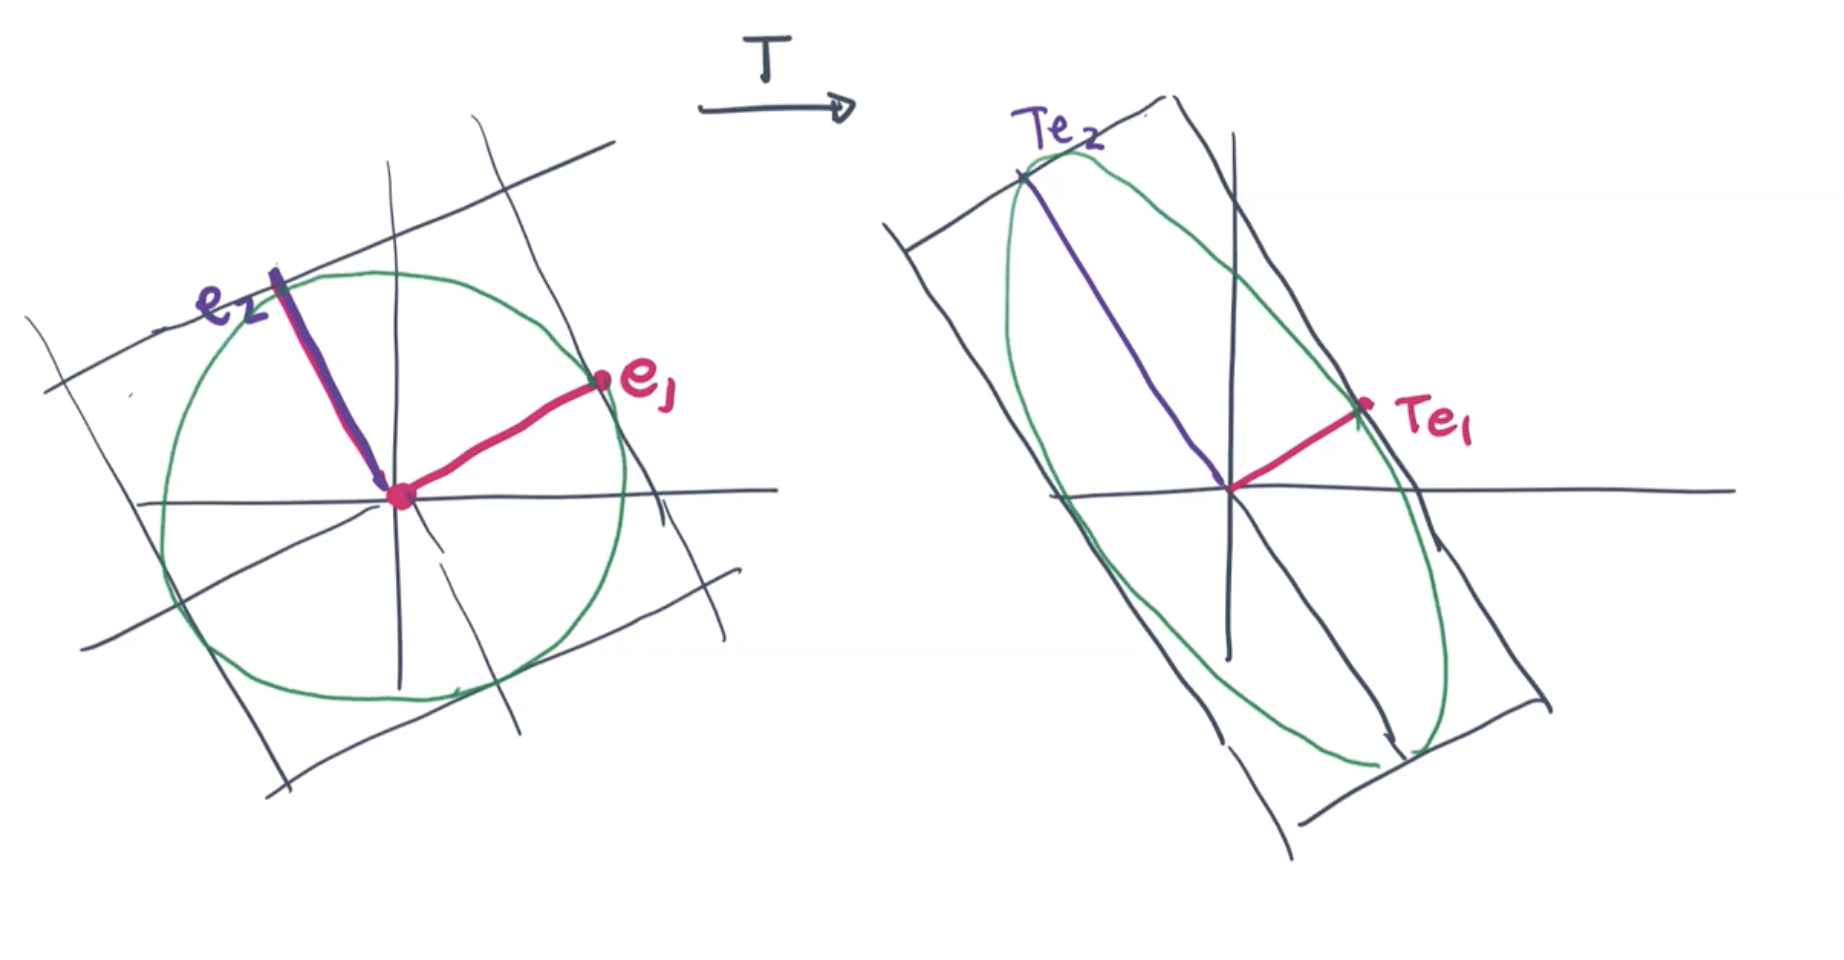
\includegraphics[width=0.5\textwidth]{last_lec.png}
\end{figure}
Note that orthogonality isn't necessarily preserved by $T$; it's simply the orthonormal bases. An
instructive example of non-positive operators is the negative identity map $-I$, or a rotation such
as a $60^{\circ}$ counter-clockwise rotation.

\begin{proposition}[Characterization of Positive Operators]{}
  Let $T\in \mc{L}(V)$. The following are equivalent:
  \begin{enumerate}
    \item $\left<Tv,v \right> \ge 0$ for all $v\in V$ and $T$ is self-adjoint.
    \item $T$ is positive ($T$ is self-adjoint and all eigenvalues are non-negative).
    \item $T$ has a positive square root.
    \item $T$ has a self-adjoint square root.
    \item There exists an operator $R\in \mc{L}(V)$ such that $T=R^*R$.
  \end{enumerate}
\end{proposition}
\begin{proof}[Proof]
  Assume $\left<Tv,v \right> \ge 0$ for all $v\in V$ and $T$ is self-adjoint. Suppose $\lambda$ is
  an eigenvalue of $T$; then \[
    \left<Tv,v \right> =\left<\lambda v,v \right> =\lambda \left<v,v \right> \ge 0
  .\] Thus any eigenvalue of $T$ is non-negative as well, proving 2 from 1.

  We prove 3 from 2. Assume $T$ is positive; then its matrix
  representation, \[
    \mc{M}(T)=\begin{pmatrix} \lambda_1&&0\\&\ddots&\\0&&\lambda_n \end{pmatrix} 
  ,\] has all non-negative eigenvalues with respect to some orthonormal basis of $V$. Since
  non-negative real numbers admit non-negative real square roots, $R\in \mc{L}(V)$ with matrix \[
    \mc{M}(R)=\begin{pmatrix} \sqrt{\lambda_1}&&0\\&\ddots&\\0&&\sqrt{\lambda_n} \end{pmatrix} 
  \] satisfies $R^2=T$. Thus $T$ has a positive square root $R$, proving 3 from 2.

  Now, assume $T$ has a positive square root. Definitionally, any positive operator is self-adjoint;
  thus 4 is true from 3.

  Now, assume $T$ has a self-adjoint square root. Then $R=R^*$, so $T=R^2=R^*R$, proving 5 from 4.

  Finally, assume an operator $R\in \mc{L}(V)$ satisfies $T=R^*R$. Then \[
    T^*=(R^*R)^*=R^*(R^*)^*=R^*R=T
  ,\] and \[
    \left<R^*Rv,v \right> =\left<Rv,Rv \right> \le 0
  \] for every $v\in V$. Thus $T$ has non-negative eigenvalues and is self-adjoint, so is positive.
\end{proof}

From mathematics, we know that every non-negative number has a unique non-negative square root. It
turns out the same is true for positive operators.
\begin{proposition}[Unique Positive Square Root]{}
  Every positive operator on $V$ has a unique positive square root.
\end{proposition}
\begin{proof}[Proof]
  [TODO: insert Axler proof]
\end{proof}

Since positive operators have unique positive square root operators, we henceforth denote the
positive square root of a positive operator $T\in \mc{L}(V)$ as $\sqrt{T}$.
\begin{mdframed}
  Note that it's not difficult to find the positive operator's positive square root; it's simply
  taking the square root of every diagonal value!
\end{mdframed}


\subsection{Isometries}

\begin{definition}[Isometries]{}
  An operator $S\in \mc{L}(V)$ is an \textbf{isometry} if \[
    \|Sv\|=\|v\|
  \] for all $v\in V$. In other words, an isometry is \textit{norm-preserving}.
\end{definition}
An intuitive way to consider isometries is via distance. Recall that we defined the ``distance''
between two vectors as its norm (recall $\R^3$'s norm). An isometry simply preserves distance.
\begin{mdframed}
  Over $\R$, isometries are called \textbf{orthogonal operators}, and over $\C$, isometries are
  called \textbf{unitary operators}. For those with group theory knowledge, orthogonal operators
  form a group; unitary operators also form a group.
\end{mdframed}

We've seen many isometries of $\R^2$; for example, all rotations and reflections are $\R^2$
(actually, that's it!) We contend that isometries also preserve ``angle'' (verify this in $\R^2$);
the following proposition formalizes this.
\begin{proposition}[Characterization of Isometries]{}
  Suppose $S\in \mc{L}(V)$. Then the following are equivalent:
  \begin{enumerate}
    \item $S$ is an isometry.
    \item $\left<Su,Sv \right> =\left<u,v \right> $ for all $u,v\in V$ ($S$ preserves ``angles'').
    \item $Se_1,\ldots,Se_n$ is orthonormal for every orthonormal list of vectors
      $e_1,\ldots,e_n\in V$.
    \item There exists an orthonormal basis $e_1,\ldots,e_n\in V$ such that $Se_1,\ldots,Se_n$ is
      orthonormal.
    \item $S^*S=S S^*=I$.
    \item $S^*$ is an isometry.
    \item $S$ is invertible and $S^{-1}=S^*$.
  \end{enumerate}
\end{proposition}
\begin{proof}[Proof]
  Suppose $S$ is an isometry. Notice that
  \begin{itemize}
    \item Over $\R$, $\left<u,v \right> =\frac{\|u+v\|^2+\|u-v\|^2}{4}$. 
    \item Over $\C$, $\left<u,v \right> =\frac{\|u+v\|^2-\|u-v\|^2+\|u+iv\|^2i-\|u-iv\|^2i}{4}$.
  \end{itemize}
  These tell us that we can completely determine inner products from norms. Since $S$ preserves
  norms, this implies that $S$ preserves inner products, and hence 1 implies 2. Concretely, if $V$
  is a real inner product space, then for every $u,v\in V$ we have
  \begin{align*}
    \left<Su,Sv \right> &= \frac{\|u+v\|^2+\|u-v\|^2}{4} \\
                        &= \frac{\|S(u+v)\|^2-\|S(u-v)\|^2}{4} \\
                        &= \frac{\|u+v\|^2-\|u-v\|^2}{4} \\
                        &=\left<u,v \right> 
  .\end{align*} A similar computation arises for complex inner product spaces. Intuitively, if the
  angles did \textit{not} stay the same, then the norms of $u+v$ and $u-v$ would change, breaking
  isometry (imagine square => parallelogram; the diagonals' lengths change).

  Now, suppose $S$ preserves inner products; in particular, it preserves orthogonality as well; thus
  3 follows from 2. 4 naturally follows from 3; simply choose an orthonormal basis, instead of just
  an orthonormal list.

  Now, say $S$ sends an orthonormal basis $e_1,\ldots,e_n$ to another orthonormal basis
  $f_1,\ldots,f_n$. We claim $S^*Se_j=e_j$ for every $e_j$. Indeed, for each $k=1,\ldots,n$, \[
    \left<S^*Se_j,e_k \right> =\left<Se_j,Se_k \right> =\left<e_j,e_k \right> 
  .\] Thus $S^*Se_j=e_j$, and so $S^*S=I$.

  We finally prove that $S$ is an isometry given 5. Given $v\in V$, we want $\|Sv\|=\|v\|$. Since \[
    \|Sv\|^2=\left<Sv,Sv \right> =\left<S^*Sv,v \right> =\left<v,v \right> =\|v\|^2
  ,\] $S$ is thus an isometry, and we are done.

  [TODO: do rest]
\end{proof}

\begin{remark}
  Indeed, if $S$ is an isometry, then $\det{\mc{M}(S)}=\pm 1$.
\end{remark}

\section{Polar Decomposition and Singular Decomposition}
\subsection{Polar Decomposition}
Recall our analogy of operators $\mc{L}(V)$ and the complex numbers $\C$. In fact, this analogy is
actually the truth, when $V=\C$!
\begin{table}[htpb]
  \centering
  \begin{tabular}{c|c}
    $\mc{L}(V)$&$\C$\\ \hline
    Adjoints & Complex conjugation\\ \hline
    Self-adjoints & $\R$\\ \hline
    Positive operators & $\R_{\ge 0}$\\ \hline
    Isometries & Unit circle in $\C: \{z\in \C\mid\|z\|=1 \} $
  \end{tabular}
\end{table}

Let's now look at polar decomposition. For any complex number $z$, we can always decompose $z$ into
a (non-negative) real number, its norm $\|z\|$, and its complex point on the unit circle,
$\frac{z}{\|z\|}$; that is, $z=(\frac{z}{\|z\|})\|z\|=(\frac{z}{\left| z \right|
})\sqrt{\overline{z}z}$ (note that in $\C$, $\|\cdot \|=\left| \cdot  \right| $). Sound familiar?

\begin{remark}
  Sometimes, $z\in C$ will be denoted $z=re^{i\theta}$, where $r=\left| z \right| $ and
  $e^{i\theta}$ is a point on the unit circle.
\end{remark}

Continuing with our analogy, it seems that we can decompose any operator $T\in \mc{L}(V)$ as an
isometry (an operator ``on the unit circle'') and $\sqrt{T^*T}$ (we can do this, since we've shown
that $T^*T$ is a positive operator, and every positive operator has a unique positive square root).
This is indeed true!
\begin{theorem}[Polar Decomposition]{}
  Suppose $T\in \mc{L}(V)$. Then there exists an isometry $S\in \mc{L}(V)$ such that \[
    T=S\sqrt{T^*T}
  .\] 
\end{theorem}

Why would we want to undergo this complicated transformation? It turns out that the polar
decomposition theorem actually tells us that singular values, defined below, hold a lot of
information about $T$.

\begin{definition}[Singular Values]{}
  For an operator $T\in \mc{L}(V)$, the \textbf{singular values} of $T$ are the eigenvalues of
  $\sqrt{T^*T}$, where each eigenvalue $\lambda$ is repeated $\dim{E(\lambda,\sqrt{T^T})}$ times.
\end{definition}
In other words, the singular values of $T$ are the diagonal entries of a diagonal matrix of
$\sqrt{T^*T}$ with respect to an orthonormal basis.\\

So, how does polar decomposition show the usefulness of singular values? For $T\in \mc{L}(V)$, polar
decomposition tells us that $T=S\sqrt{T^*T}$ for some isometry $S$. Then for an orthonormal basis
$e_1,\ldots,e_n$ (for instance, the standard basis in $\R^2$), we have:
\begin{figure}[htpb]
  \centering
  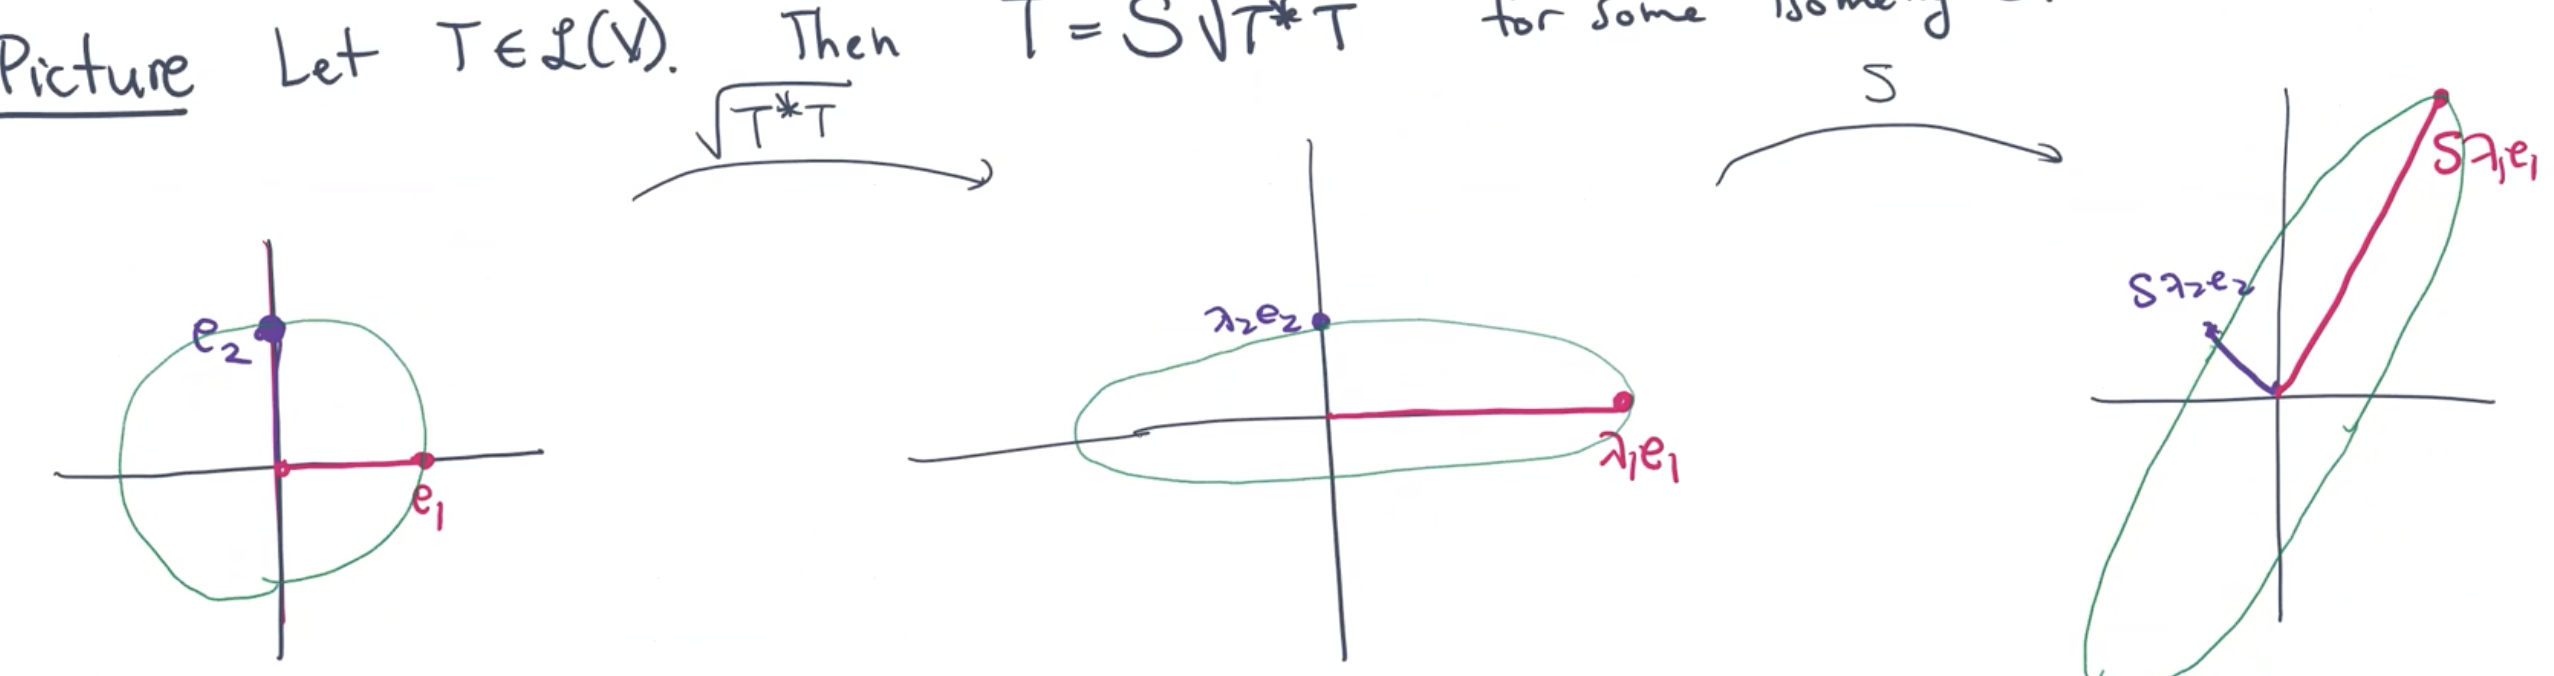
\includegraphics[width=0.75\textwidth]{last_lec2.png}
\end{figure}
\\
In other words, for any arbitrary operator $T\in \mc{L}(V)$, we can decompose it into two operators:
one that ``stretches'' its eigenvalues (\textbf{these are the singular values}), and one that
preserves the norms (e.g. rotations/reflections in $\R^2$).\\

Now that we somewhat understand the usefulness of this decomposition, let's prove it.
\begin{proof}[Proof]
  We start with a lemma:
  \begin{lemma}{}
    For all $v\in V$, \[
      \|Tv\|=\|\sqrt{T^*T}v\|
    .\] 
  \end{lemma}
  \begin{proof}[Proof]
    If $v\in V$, then
    \begin{align*}
      \|Tv\|^2=\left<Tv,Tv \right> &= \left<T^*Tv,v \right>  \\
      &= \left<\sqrt{T^*T}\sqrt{T^*T}v,v \right>  \\
      &= \left<\sqrt{T^*T}v,\sqrt{T^*T}v \right>  \\
      &=\|\sqrt{T^*T}v\|^2
    .\end{align*}
    Thus \[
      \|Tv\|=\|\sqrt{T^*T}v\|~\text{for all}~v\in V
    ,\] as desired.
  \end{proof}
  
  This is promising; since the norms of the square root $\sqrt{T^*T}$ and $T$ are preserved for any
  $v\in V$, an isometry is possible. Let's sketch a high-level outline of the proof:
  \begin{enumerate}
    \item Define a linear map \[
        S_1:\range{(\sqrt{T^*T})}\longrightarrow \range{T},\ S_1(\sqrt{T^*T})=Tv
      .\] Recall our original goal: if we wish for the decomposition to hold, we must be able to
      define an isometry that maps $S(\sqrt{T^*T}v)\mapsto Tv$. We use $S_1$ to make such an
      isometry. However, we need to check that this linear map is well-defined; that is, if
      $v_1,v2\in V$ with $\sqrt{T^*T}v_1=\sqrt{T^*T}v_2$, then $Tv_1=Tv_2$.
    \item Then, we wish to extend the linear map $S_1$ to an isometry $S\in \mc{L}(V)$ such that
      $T=S\sqrt{T^*T}$, since currently $S_1$ only maps $\range{(\sqrt{T^*T})}$ to $\range{T}$.
      Luckily, we can do this by sending an orthonormal basis of $(\range{\sqrt{T^*T}})^\bot$ to an
      orthonormal basis of $(\range{T})^\bot$, and we're done (since every vector space decomposes
      into a subspace and its orthogonal complement)!
  \end{enumerate}

  Now, for the details. We first check that the map \begin{align*}
    S: \range{(\sqrt{T^*T})} &\longrightarrow \range{T} \\
    \sqrt{T^*T}v &\longmapsto Tv
  \end{align*} is well-defined.
  
\end{proof}







\end{document}
